\chapter{Linear,Quadratic, Polynomial and Rational Functions}
\author{Nithin}

\section{Lines and Linear Function}
\subsection{Slope}
\begin{figure}
  \centering
  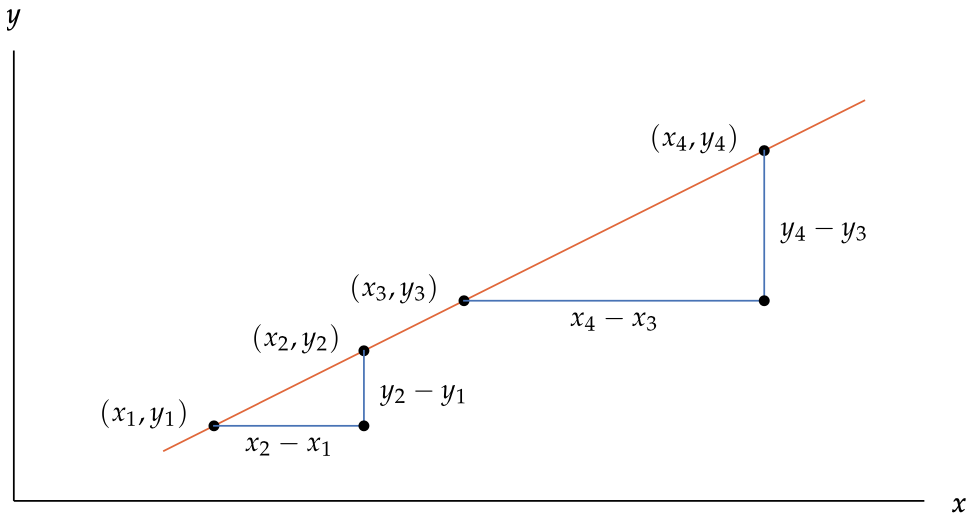
\includegraphics[scale=0.25]{slope.png}
\end{figure}
\[\frac{y_{2} - y_{1}}{x_{2} - x_{1}} = \frac{y_{4} - y_{3}}{x_{4} - x_{3}}\]

If \(x_{1},y_{1}\) and \(x_{2},y_{2}\) are any two points on a line with \(x_{1} \neq x_{2}\), then the \textbf{slope} of the line is
\[\frac{y_{2} - y_{1}}{x_{2} - x_{1}}\]

\begin{figure}
  \centering
  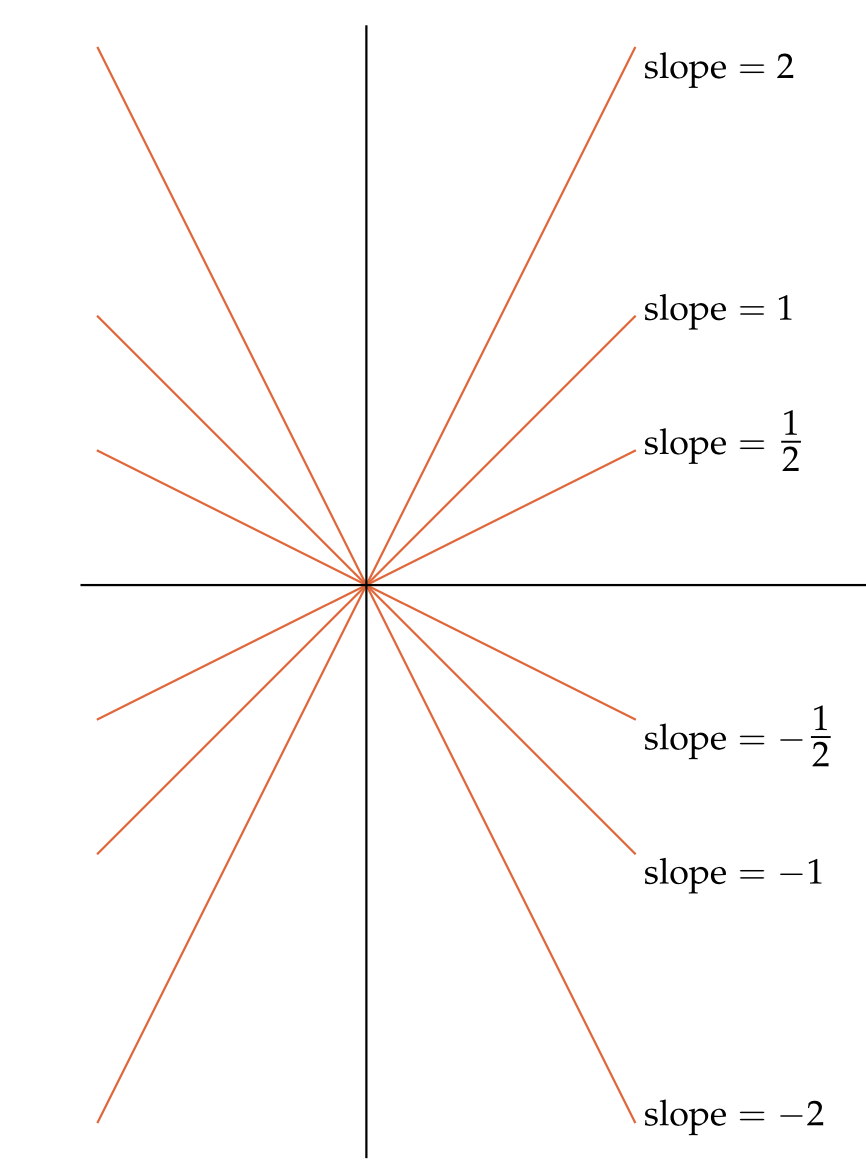
\includegraphics[width=0.5\linewidth]{slope2.png}
\end{figure}
\textbf{Key Points:}
\begin{itemize}
    \item Positive slope slands up from left to right
    \item Negative slope slands down from left to right
    \item Horizontal line has slope = 0
    \item Vertical line has no slope
\end{itemize}

\subsection{Line Equation}
\subsubsection{Slope and one point on it}
The line in the xy-plane that has slope \(m\) and contains the point \((x1, y1)\) is given by the equation
\[y - y_{1} = m(x  -  x_{1})\]
\begin{figure}
  \centering
  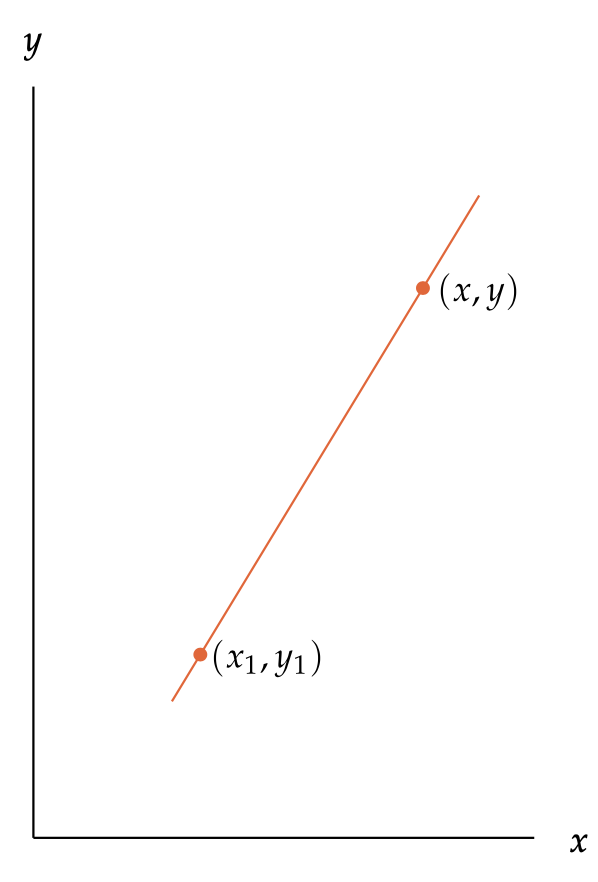
\includegraphics[width=0.5\linewidth]{line1.png}
\end{figure}

\subsubsection{Slope and \(y\) intercept}
The line in the xy-plane with slope \(m\) that intersects the \(y\) axis at \(0,b\) is given by the equation
\[y = mx+b\]
\begin{figure}
  \centering
  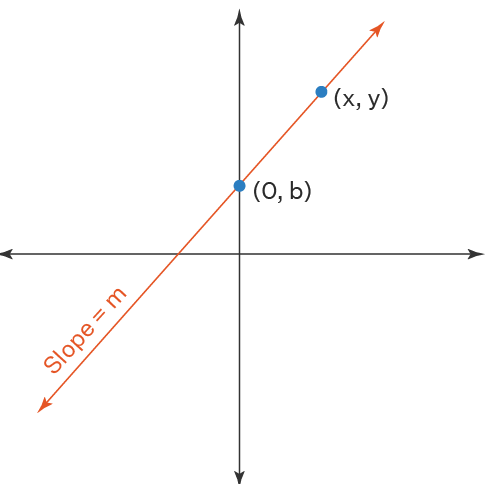
\includegraphics[width=0.5\linewidth]{line2.png}
\end{figure}

The line in the xy-plane that contains the points \(x_{1},y_{1}\) and \(x_{2}, y_{2}\) where \(x_{1} \neq x_{2}\), is
\[y-y_{1} = \left( \frac{y_{2} - y_{1}}{x_{2} - x_{1}} \right) (x-x_{1})\]

\subsection{Linear Function}
A \textbf{linear function} is a function \(f\) of the form
\[f(x) = mx + b\]
where \(m\) and \(b\) are numbers.

\subsubsection{Linear Functions: Origin vs Y-Intercept}
\textbf{Example 1: Temperature Conversion}
\begin{itemize}
    \item Correct formula: \( F = 1.8C + 32 \) (Starts at 32°F)
    \item Incorrect direct proportion: \( F' = 1.8C \) (Wrong assumption)
\end{itemize}
\textbf{Example 2: Weight Conversion}
\begin{itemize}
    \item True conversion: \( lb = 2.205 \times kg \) (Passes through origin)
    \item Shipping charge model: \( lb' = 5 + 2.205 \times kg \) (Has minimum billable weight or fixed cost markup)
\end{itemize}
\begin{figure}
\centering
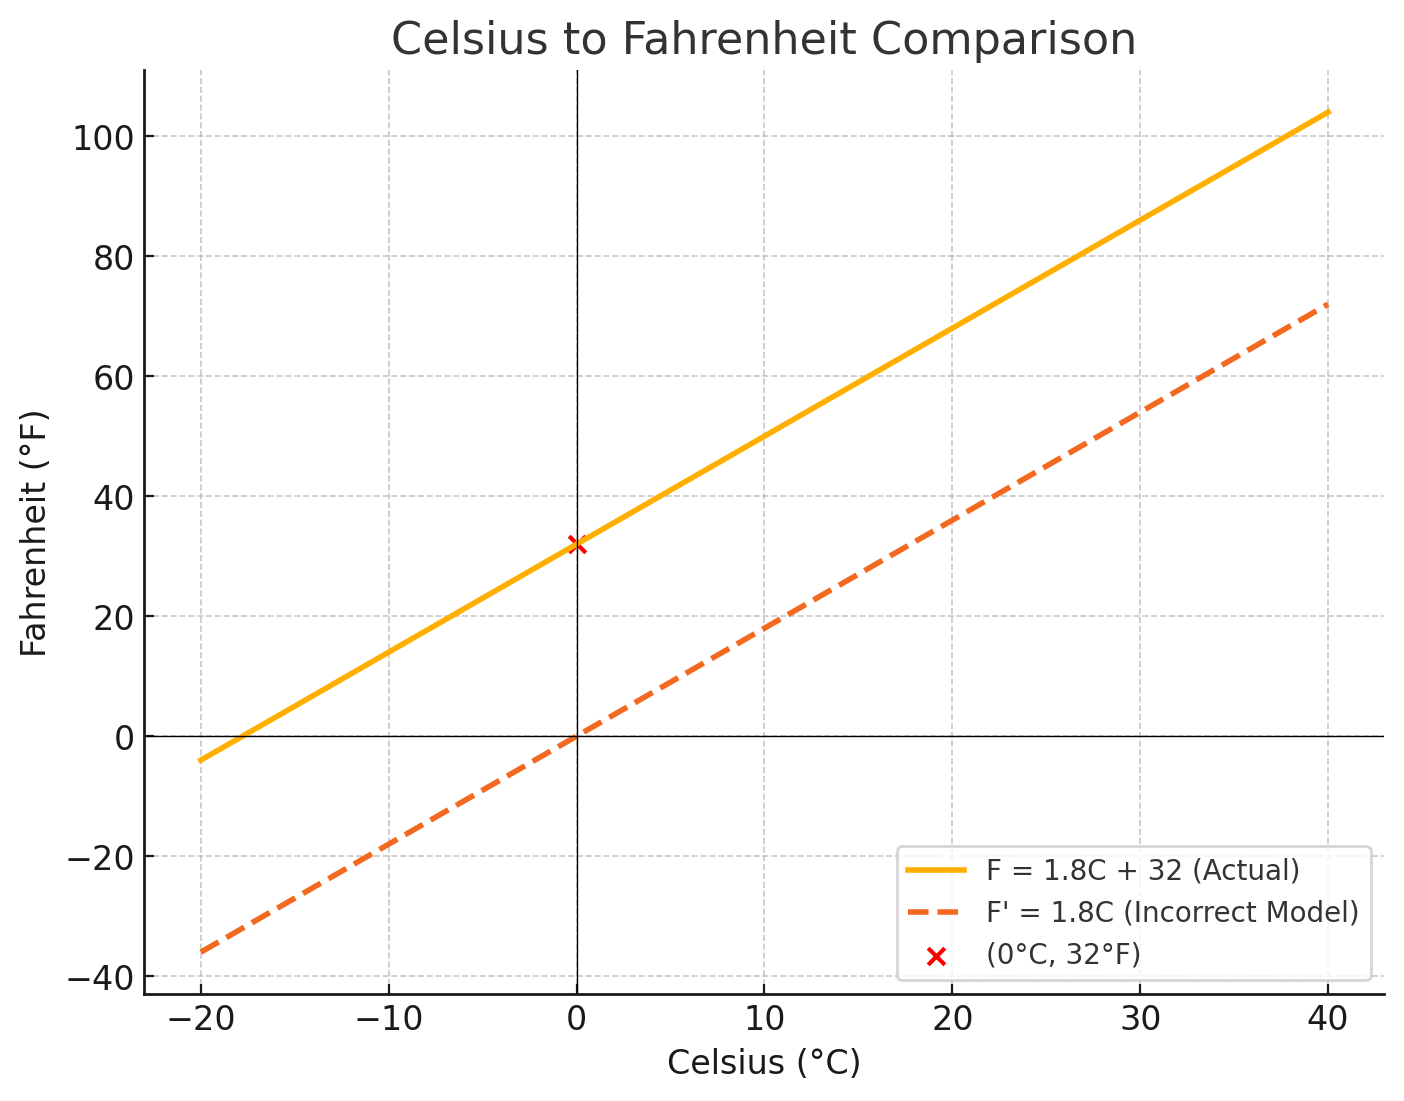
\includegraphics[width=0.45\linewidth]{Celsius to Fahrenheit Comparison.png}
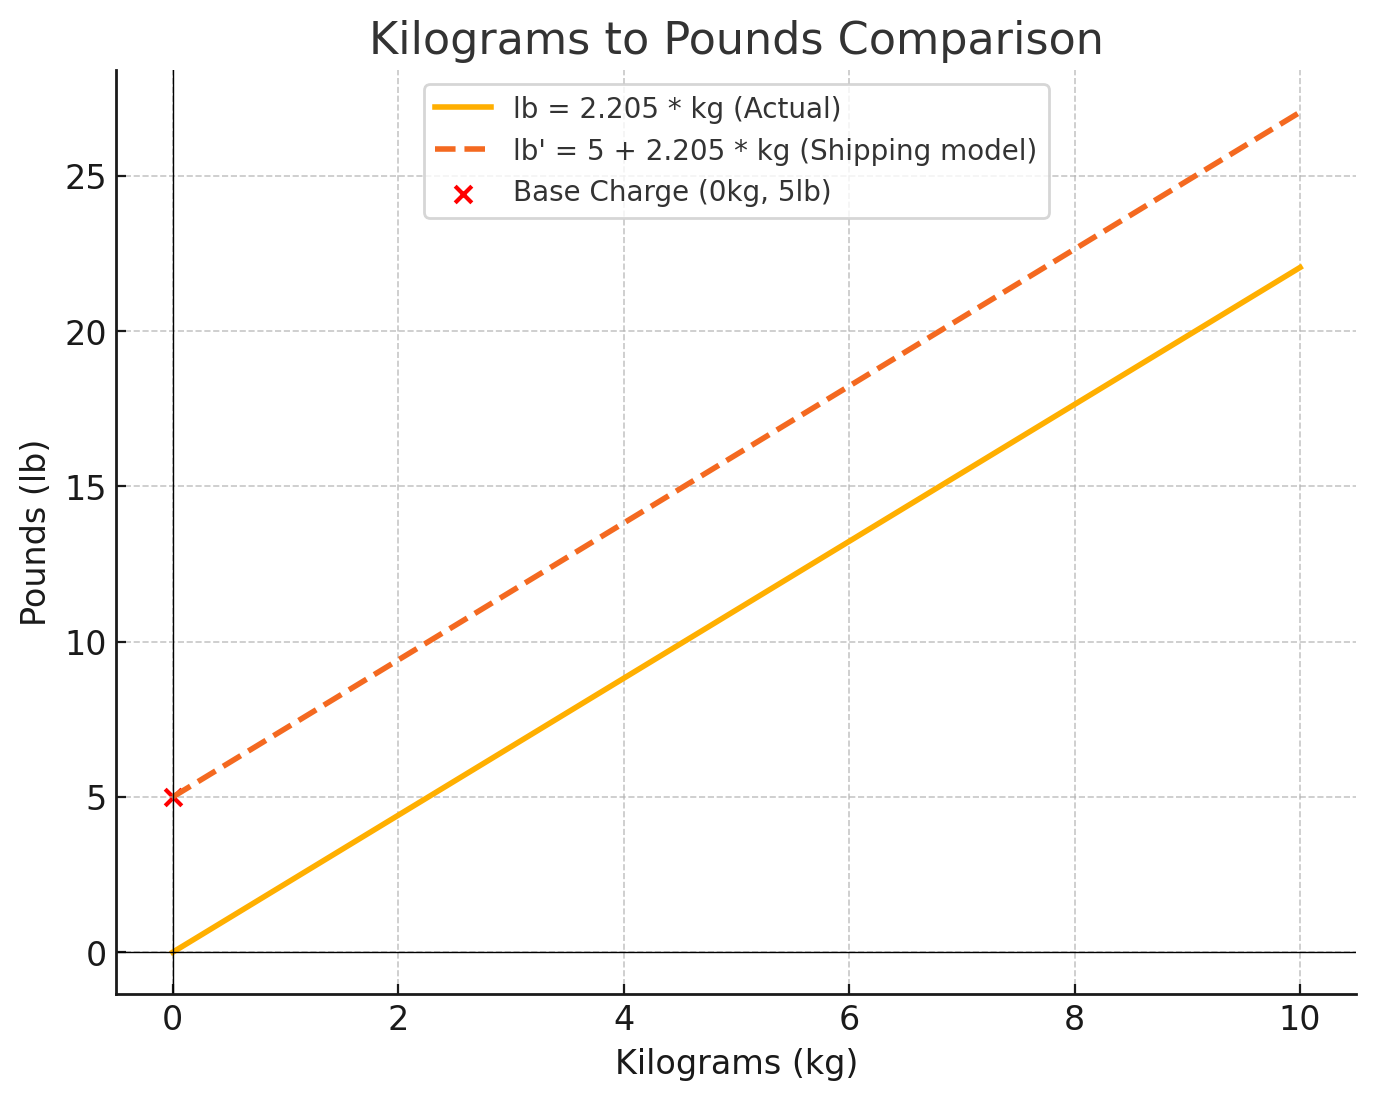
\includegraphics[width=0.45\linewidth]{Kilograms to Pounds Comparison.png}
\end{figure}

\subsection{Constant Function}
A constant function is a function \(f\) of the form \(f (x) = b\),  where \(b\) is a number.
\begin{figure}
\centering
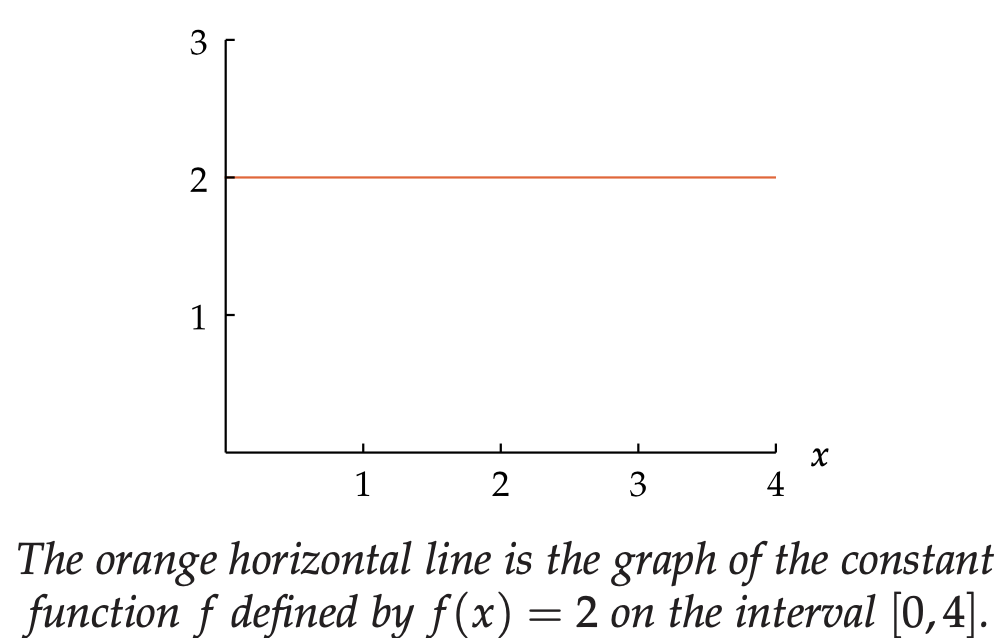
\includegraphics[width=0.6\linewidth]{constant.png}
\end{figure}

\subsection{Parallel Lines}
\begin{figure}
  \centering
  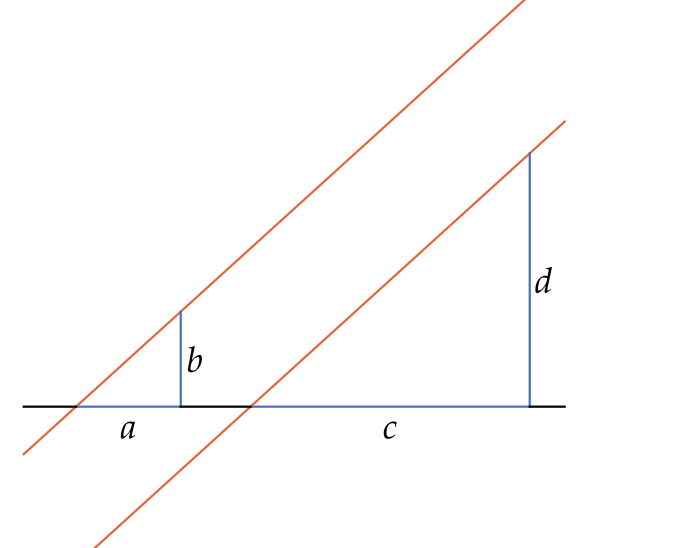
\includegraphics[scale=0.2]{parallel.png}
\end{figure}
As two lines are parallel, the corresponding angles are concurent and so two triangles are similar so
\[\frac{a}{c} = \frac{b}{d} \implies \frac{b}{a} = \frac{d}{c}  \]
it has same slope.

\subsection{Negative Slope}
\begin{figure}
  \centering
  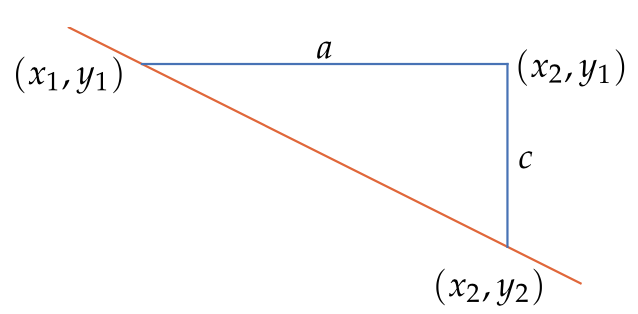
\includegraphics[scale=0.3]{negative-slope.png}
\end{figure}
As lengths are positive \(a = x_{2} - x_{1}\) and \(c = y_{1} - y_{2} \)
Slope  = \(\frac{y_{2} - y_{1}}{x_{2} - x_{1}} = -\frac{c}{a} \

\subsection{Perpendicular Lines}
\begin{figure}
  \centering
  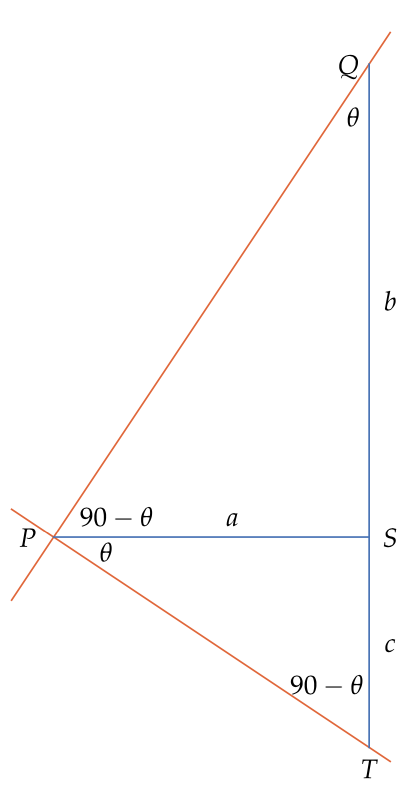
\includegraphics[width=0.5\linewidth]{perpendicular.png}
\end{figure}
\(\triangle PSQ \) and \( \triangle TSP \) are similar
\(\frac{QS}{SP} = \frac{PS}{ST} \implies \frac{b}{a} = \frac{a}{c} \
Multiplying by \(-\frac{c}{a} \implies \frac{b}{a} \cdot \left( - \frac{c}{a} \right) = -1  \

\subsection{Unequal Scales}
Angles are distorted by unequal scales on coordinate axes. In graphs with unequal scales on the two coordinate axes, angles are not accurately represented.
\begin{figure}
  \centering
  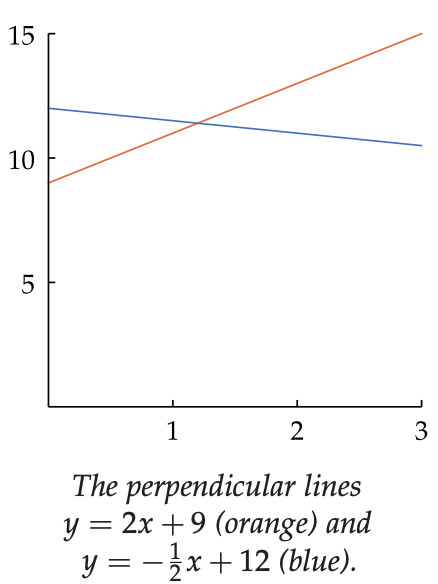
\includegraphics[scale=0.25]{unequal-scale.png}
\end{figure}

\section{Quadratic Functions and Conics}
\subsection{Conics}
\begin{figure}
  \begin{center}
    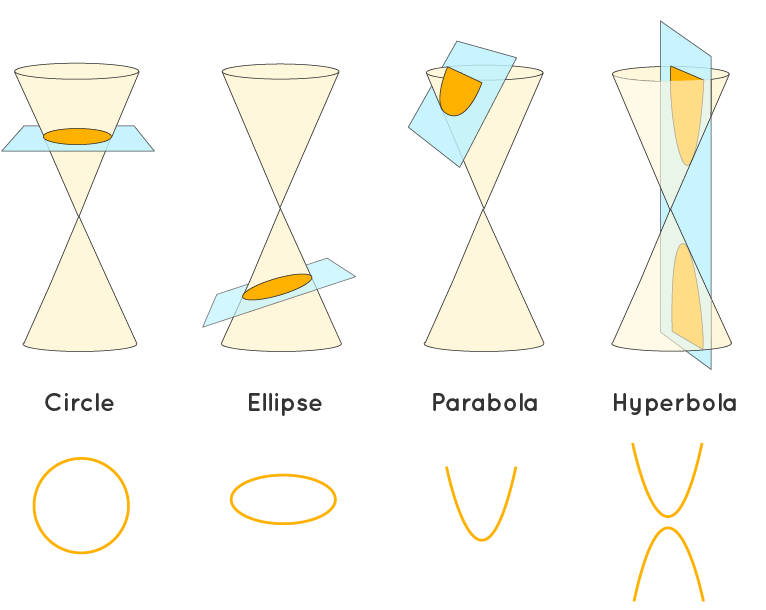
\includegraphics[scale = 0.3]{conic-section.png}
  \end{center}
\end{figure}

\subsection{Quadratic Function}
The function of the form
\[ax^{2} + bx + c = 0\]
where \(a,b,c\) are real numbers with \(a \neq 0\)
\begin{itemize}
    \item if \(b^{2} - 4ac < 0\), then equation have no real solutions
    \item if \(b^{2} - 4ac = 0\), then equation has one solution, \(x = -\frac{b}{2a}\)
    \item if \(b^{2} - 4ac  > 0\), then equation has two solutions \(x = \frac{-b \underset{-}{+}\sqrt{b^{2} - 4ac}}{2a}
\end{itemize}

\subsection{Parabola}
A \textbf{parabola} is the graph of a quadratic function. The \textbf{vertex} of the parabola is the where the line of symmetry of the parabola, intersects the parabola.
Suppose \(f\) is a quadratic function. Complete the square to write \(f\) in the form
\[ f(x) = a(x-h)^{2} + k \
\begin{itemize}
    \item If \(a > 0\) then \(f(x)\) attains its minimum value \(k\) when \(x=h\) and the graph of \(f\) is a parabola that opens upward.
    \item If \(a < 0 \) then \(f(x) \) its maximum value \(k\) when \(x=h\) and the graph of \(f\) is a parabola that opens downward
    \item The vertex of the graph is \(h,k\)
\end{itemize}

\subsubsection{Example}
\[f(x) = -3x^{2} + 12x - 8 \
\begin{enumerate}
  \item For what value of \(x\) does \(f (x) \) attain its maximum value?
  \item What is the maximum value of \(f (x)\)?
  \item Find the vertex
\end{enumerate}
Sol:
\[f(x) = -3x^{2} + 12x - 8 \implies -3(x^{2} - 4x + 4) + 4 \implies -3(x-2)^{2} + 4 \
\begin{enumerate}
\item \(x = 2\
\item \(f(x=2) = 4\
\item \( (2,4) \
\end{enumerate}

\begin{figure}
\centering
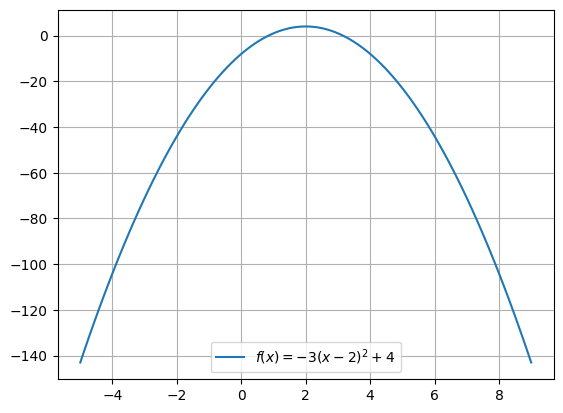
\includegraphics[scale=0.6]{parabola.png}
\end{figure}

\subsection{Distance Between Points}
\begin{figure}
\centering
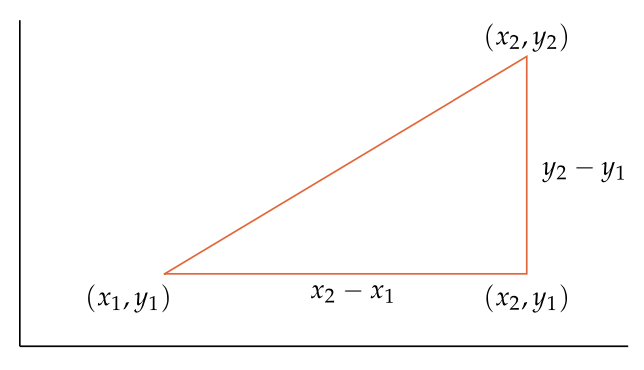
\includegraphics[scale=0.3]{distance-between-points.png}
\end{figure}
The distance between points \(x_{1}, y_{1}\) and \(x_{2}, y_{2}\) is given by
\[\sqrt{ \left(x_{2} - x_{1} \right)^{2}  + \left( y_{2} - y_{1} \right)^{2} }\]

\subsection{Circle}
The circle with center \(h,k\) and radius \(r\) is the set of the points \(x,y\) that satisfy the equation
\[\left(x-h\right)^{2} + \left(y-k\right)^{2} = r^{2}\]

\subsection{Ellipse}
\begin{figure}
\centering

\includegraphics[scale=0.38]{ellipse0.png}
\end{figure}

Stretching the circle horizontally and/or vertically produces a curve called an \textbf{ellipse}.
\begin{figure}
\centering
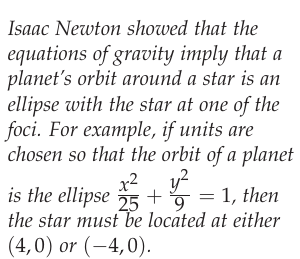
\includegraphics[scale=0.4]{ellipse1.png}
\end{figure}

\subsubsection{Example}
Equation of the circle is given by \(u^{2} + v^{2} = 1\).
By stretching \(x = 3u, y = 5v\),
Substituting for \(u,v\)
\[ \left( \frac{x}{3} \right)^{2} + \left(\frac{y}{5}\right)^{2} = 1 \

\subsubsection{Ellipse Equation}
\[\frac{x{2}}{a^{2}} + \frac{y^{2}}{b^{2}} = 1 \
The \textbf{foci} of an ellispe are two points with the property that the sum of the distances from the \textbf{foci} to any point on the ellipse is a constant independent of the point on the ellispe.

\begin{figure}
\centering
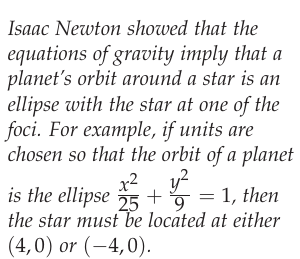
\includegraphics[scale=0.5]{ellipse1.png}
\end{figure}

\begin{figure}
\centering
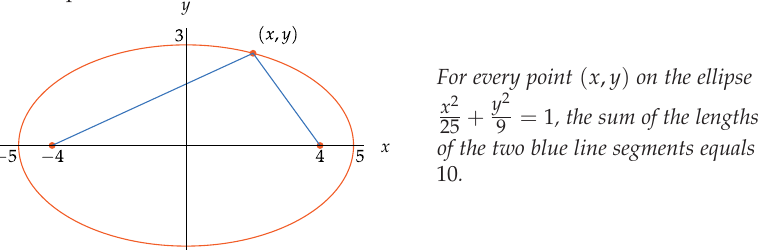
\includegraphics[scale=0.4]{foci.png}
\end{figure}

\subsection{Eccentricity of an Ellipse}
The \textbf{eccentricity} (\(e\)) of an ellipse is a measure of how much the ellipse deviates from being a circle. It is defined as
\[ e = \frac{c}{a} .
\qquad c^2 = a^2 - b^2, 
\qquad e = \sqrt{1 - \frac{b^2}{a^2}}\]
where:
\begin{itemize}
    \item \(c\) is the distance from the center to a focus.
    \item \(a\) is the length of the semi-major axis.
\end{itemize}
Additionally, the semi-minor axis \(b\) is related to \(a\) and \(c\) by:
\textbf{Key Points:}
\begin{itemize}
    \item If \(e = 0\), the ellipse is a circle.
    \item If \(0 < e < 1\), the ellipse is elongated, with greater elongation as \(e\) increases.
\end{itemize}

\subsection{Hyperbola}
The graph of the equation of the form
\[ \frac{y^2}{b^2} - \frac{x^2}{a^2} = 1 \
where \(a,b\) are non-zero numbers.
\begin{figure}
\centering
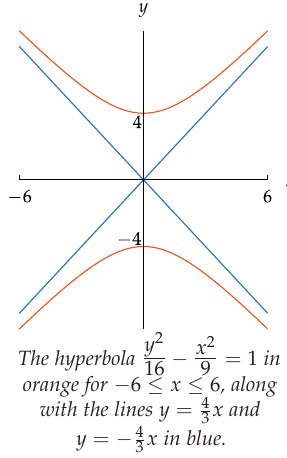
\includegraphics[scale=0.5]{hyperbola2.png}
\end{figure}

The foci of a hyperbola are two points with the property that the difference of the distances from the foci to a point on the hyperbola is a constant independent of the point on the hyperbola.
\begin{figure}
\centering
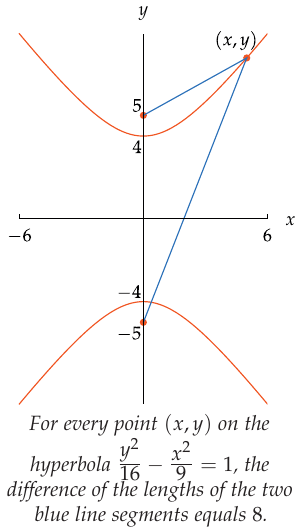
\includegraphics[scale=0.4]{hyperbola3.png}
\end{figure}
\begin{figure}
\centering
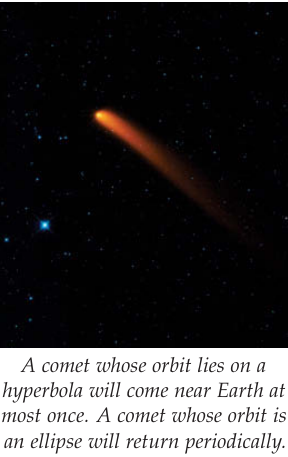
\includegraphics[scale=0.5]{hyperbola1.png}
\end{figure}

\section{Exponents}
\subsection{Positive Integer Exponent}
If \(x\) is a real number and \(m\) is a positive integer, then \(x^{m}\) is defined to be the product with \(x\) appearing \(m\) times
\[x^{m} = \underset{x \;	ext{appears}\;	ext{m} \;	ext{times}}{\underbrace{x \cdot x \cdots x }}\]

\subsubsection{Properties}
Suppose \(x\) and \(y\) are numbers and \(m\) and \(n\) are positive integers. Then
\[x^{m}x^{n} = x^{m+n} \
\left(x^{m}\right)^{n} = x^{mn} \
x^{m}y^{m} = \left(xy\right)^{m}\]

\subsection{\(x^{0}\)}
If  \(x^{m}x^{n} = x^{m+n}\) then we can write \(x^{0}x^{n} = x^{0+n} = x^{n} \implies x^{0} = 1\;for\;	ext{x} \neq 0\]

\subsubsection{What is \(0^{0}\)}
\begin{itemize}
  \item The rule \( x^0 = 1 \) (for \( x \neq 0 \)) suggests that \( 0^0 \) should be \(1\).
  \item The rule \( 0^m = 0 \) (for \( m > 0 \)) suggests that \( 0^0 \) should be \(0\).
  \item Since these two rules contradict each other, \( 0^0 \) is left undefined in general mathematics.
  \item However, in combinatorics and programming, \( 0^0 \) is often defined as \(1\) for convenience.
\end{itemize}

\subsection{Negative Integer Exponents}
If \(x^{m}x^{n} = x^{m+n}\), if we take \(m = -n \), then
\[x^{m}x^{-m} = x^{0} = 1 \implies x^{m}x^{-m} = 1\]
We have to define \(x^{-m}\) to equal the multiplicative inverse of \(x^{m}\).
If \(x \neq 0\) and \(m\) is a positive integer, then \(x^{-m}\) is defined to multiplicative inverse of \(x^{m}\)
\[x^{-m} = \frac{1}{x^{m}}\]

\subsubsection{Exponents: Some Graphs}
\begin{figure}
\centering
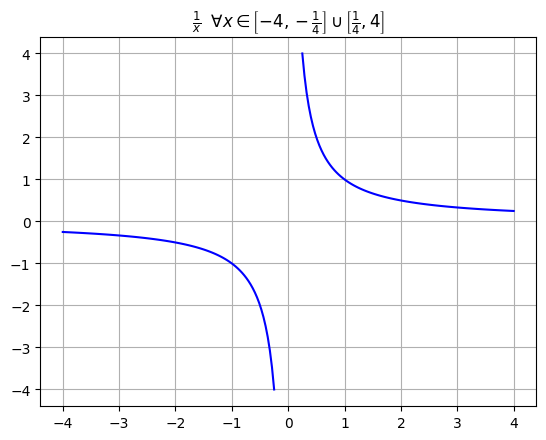
\includegraphics[scale=0.4]{exponent-graph1.png}
\caption{graph of \(\frac{1}{x}\)}
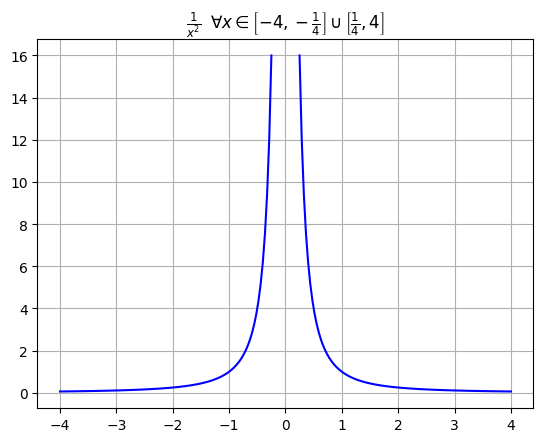
\includegraphics[scale=0.4]{exponent-graph2.png}
\caption{graph of \(\frac{1}{x^{2}}\)}
\end{figure}

\subsubsection{Graph of Negative Integer Exponents}
if \(m\) is  a positive integer then
\begin{itemize}
  \item \(\frac{1}{x^{m}}\) behaves like \(\frac{1}{x}\) if \(m\) is odd
  \item \(\frac{1}{x^{m}}\) behaves like \(\frac{1}{x^{2}}\) if \(m\) is even
  \item Larger values of \(m\) correspond to functions whose graphs get closer to the x-axis more rapidly for large values of \(x\) and closer to the vertical axis more rapidly for values of \(x\) near 0
\end{itemize}

\subsection{Roots}
\subsubsection{\(m^{th}\) root}
If \(m\) is a positive integer and \(x\) is a real number, then \(x^{m}\) is defined to be the real number satisfying the equation
\[\left(x^{m}\right)^{m} = x \
subject to the following conditions:
\begin{itemize}
\item  If \(x < 0\) and \(m\) is an even integer, then \(x^{m} \)is undefined
\item If \(x > 0\) and \(m\) is an even integer, then \(x^{m} \)is chosen to be the \textit{\textcolor{red}{positive number}} satisfying the equation above
\end{itemize}
The number \(x^{m}\) is called the \textbf{\(m^{th}\)} root of \(x\).

\subsubsection{Example}
\begin{itemize}
  \item \(8^{3}\) and \(-8^{3}\)
  \item \(9^{2}\) and \(-9^{2}\)
\end{itemize}
Solution:
\begin{enumerate}
  \item \( \left(8^{3}\right)^{3} = 8 \implies 2 \
  \item \( \left(-8^{3}\right)^{3} = -8 \implies -2 \). There is no other number other than \(-2\)
  \item \( \left( 9^{2} \right)^{2} = -3 \; or \;3\). But as per the rule, we have to choose positive possibility, that is \(3\
  \item \( \left( -9^{2} \right)^{2} \). No number real number exists so no solution
\end{enumerate}

\subsection{Rational Exponents}
Suppose \(\frac{n}{m}\) is a fraction in reduced form, where \(n\) and \(m\) are integers and \(m > 0\). Then, whenever it makes sense,
\[ x^{\frac{n}{m}} = \Bigl(x^{\frac{1}{m}}\Bigr)^n. \
\textbf{Note:} For the expression \(x^{\frac{1}{m}}\) to be defined, additional conditions on \(x\) may be required (for example, if \(m\) is even, then typically \(x \ge 0\)).

\subsection{Algebra of Exponents}
Let \(p, q\) be rational numbers and \(x, y\) be positive numbers. Then the following rules hold:
\begin{itemize}
  \item \(x^p \cdot x^q = x^{\,p+q}
  \item \(x^p \cdot y^p = (xy)^p
  \item \((x^p)^q = x^{\,pq}
  \item \(x^0 = 1
  \item \(x^{-p} = \dfrac{1}{x^p}
  \item \(\dfrac{x^p}{x^q} = x^{\,p-q}
  \item \(\left(\dfrac{x}{y}\right)^p = \dfrac{x^p}{y^p}
\end{itemize}

\section{Polynomials}
\subsection{Polynomial Definition}
A polynomial is a function \( p \) such that
\[ p(x) = a_0 + a_1 x + a_2 x^2 + \cdots + a_n x^n, \
where \( n \) is a nonnegative integer and \( a_0, a_1, a_2, \dots, a_n \) are numbers.

\subsection{Degree of a Polynomial}
Suppose \( p \) is a polynomial defined by
\[ p(x) = a_0 + a_1 x + a_2 x^2 + \cdots + a_n x^n. \
If \( a_n \neq 0 \), then we say that \( p \) has degree \( n \). The degree of \( p \) is denoted by \(\deg p\).

\subsection{Polynomial Graphs}
\begin{figure}
\centering
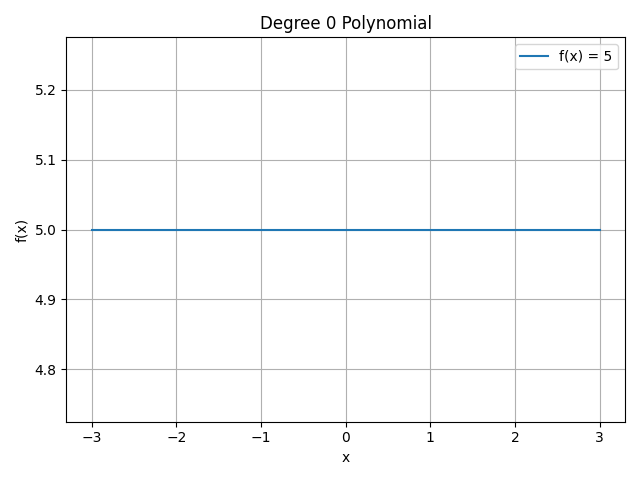
\includegraphics[width=0.45\linewidth]{polynomial_degree_0.png}
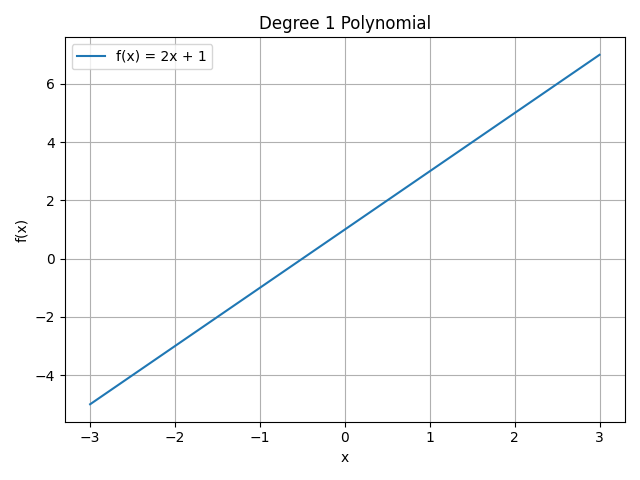
\includegraphics[width=0.45\linewidth]{polynomial_degree_1.png}
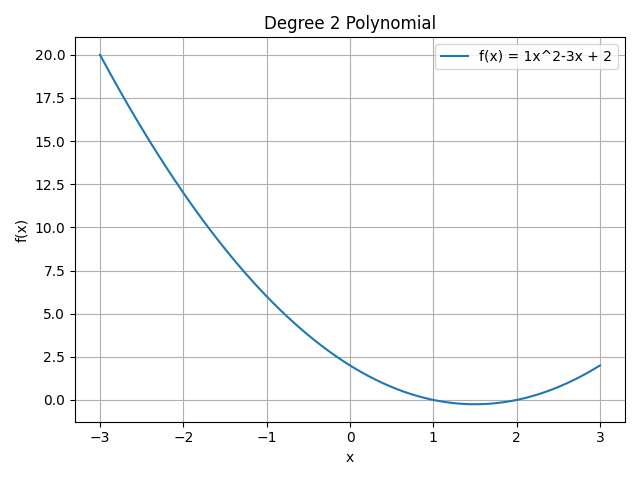
\includegraphics[width=0.45\linewidth]{polynomial_degree_2.png}
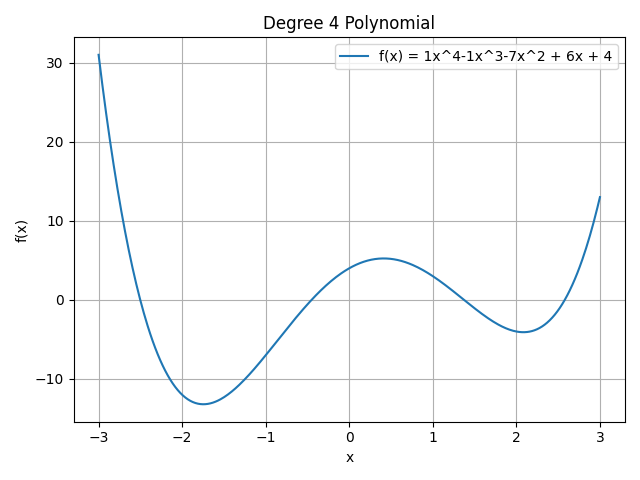
\includegraphics[width=0.45\linewidth]{polynomial_degree_4.png}
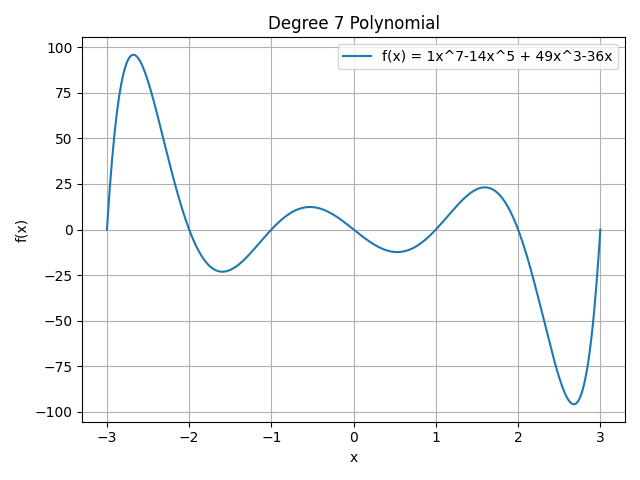
\includegraphics[width=0.45\linewidth]{polynomial_degree_7.png}
\end{figure}

\subsection{The Algebra of Polynomials}
Two functions can be added, subtracted, or multiplied, producing another function. Specifically, if \(p\) and \(q\) are functions, then the functions
\[ p+q,\quad p-q,\quad \text{and} \quad pq \
are defined by
\[ (p+q)(x) = p(x) + q(x), \
\[ (p-q)(x) = p(x) - q(x), \
\[ (pq)(x) = p(x) \, q(x). \

\subsection{Degree of the Sum and Difference of Two Polynomials}
If \(p\) and \(q\) are nonzero polynomials, then
\[ \deg(p+q) \leq \max\{\deg p,\, \deg q\}, \
and
\[ \deg(p-q) \leq \max\{\deg p,\, \deg q\}. \

\subsection{Degree of the Product of Two Polynomials}
If \(p\) and \(q\) are nonzero polynomials, then
\[ \deg(pq) = \deg p + \deg q. \

\subsection{Example: Polynomials \(p\) and \(q\)}
Suppose \(p\) and \(q\) are polynomials defined by
\[ p(x) = 2 - 3x^2 \quad \text{and} \quad q(x) = 4x + 7x^5. \
Answer the following:
\begin{enumerate}
    \item What is \(\deg p\)?
    \item What is \(\deg q\)?
    \item Find a formula for \(pq\).
    \item What is \(\deg(pq)\)?
\end{enumerate}
Solution:
\begin{enumerate}
    \item Since \(p(x) = 2 - 3x^2\) has the highest power \(x^2\), we have \(\deg p = 2\).
    \item For \(q(x) = 4x + 7x^5\), the highest power is \(x^5\), so \(\deg q = 5\).
    \item The product \(pq\) is computed as follows:
    \[ pq = (2-3x^2)(4x+7x^5) = 2\cdot 4x + 2\cdot 7x^5 - 3x^2\cdot 4x - 3x^2\cdot 7x^5, \
    which simplifies to:
    \[ pq = 8x - 12x^3 + 14x^5 - 21x^7. \
    \item The highest power in \(pq\) is \(x^7\), so \(\deg(pq) = 7\).
\end{enumerate}

\subsection{Roots of a Function}
A number \(t\) is called a zero of a function \(p\) if
\[ p(t) = 0. \

\subsection{Closed-Form Expression}
A closed-form expression is an explicit formula that can be written using a finite number of standard operations and functions (e.g., addition, multiplication, exponentiation, logarithms, trigonometric functions). It does not involve infinite series, integrals, or iterative processes.
\textbf{Example:} The quadratic formula,
\[ x = \frac{-b \pm \sqrt{b^2-4ac}}{2a}, \
is a closed-form expression.

\subsection{Zeros of Higher–Degree Polynomials}
\begin{itemize}
  \item The quadratic formula gives exact zeros for degree–2 polynomials.
  \item Although formulas exist for cubics and quartics, they are rarely used.
  \item No closed-form formula exists for polynomials of degree 5 or higher.
  \item Numerical methods can approximate zeros for any polynomial.
  \item \textbf{Example:} For
  \[ p(x)=x^5-5x^4-6x^3+17x^2+4x-7, \
  approximate zeros are:
  \[ -1.80,\; -0.73,\; 0.63,\; 1.48,\; 5.56. \
\end{itemize}

\subsubsection{Zeros on graph}
\begin{figure}
\centering
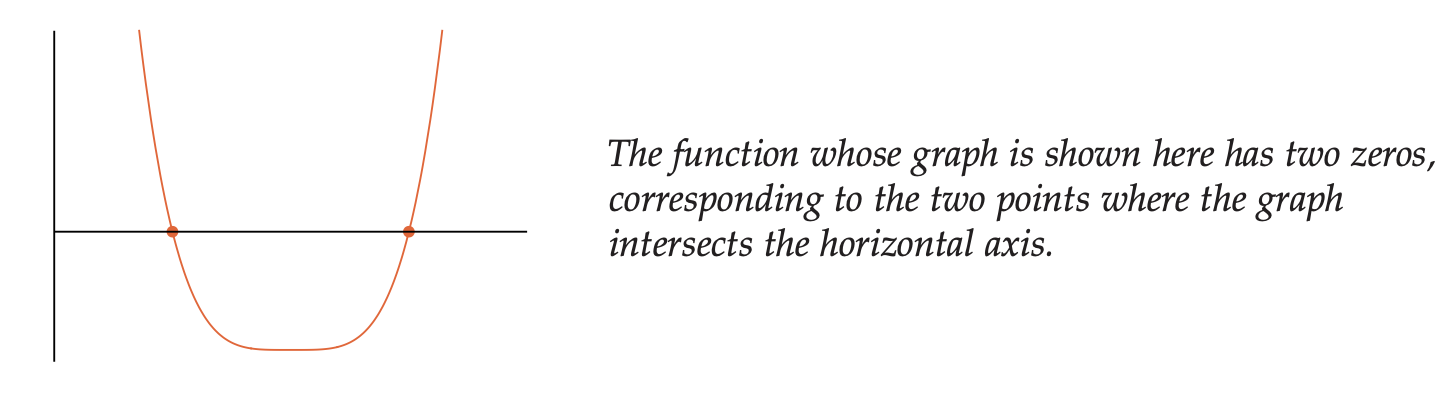
\includegraphics[scale=0.23]{zeros.png}
\end{figure}
\begin{figure}
\centering
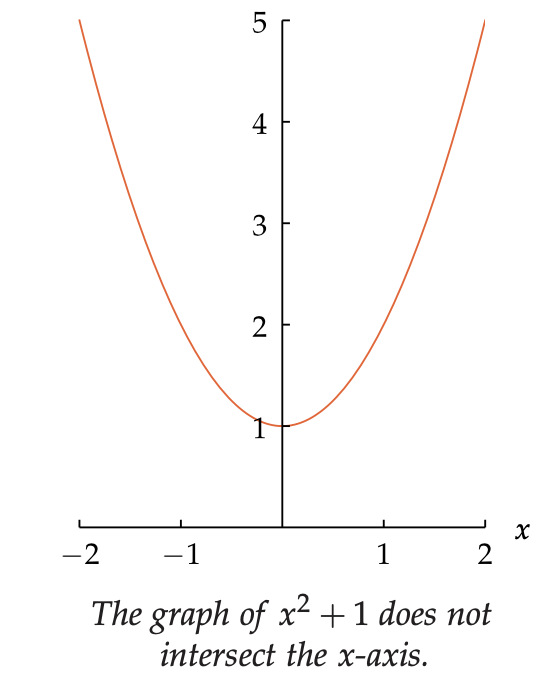
\includegraphics[scale=0.3]{no-real-zeros.png}
\caption{The function \(x^{2}+1\) has no real zeros}
\end{figure}

\subsection{Factor of a Polynomial}
Suppose \(p\) is a polynomial and \(t\) is a real number. Then \(x-t\) is called a \emph{factor} of \(p(x)\) if there exists a polynomial \(G(x)\) such that
\[ p(x) = (x-t)\,G(x) \
for every real number \(x\).

\subsection{Example: Factors and Zeros of a Polynomial}
Let
\[ p(x) = (x-2)(x-5)(x^2+1). \
\begin{enumerate}[(a)]
  \item Explain why \(x-2\) is a factor of \(p(x)\).
  \item Explain why \(x-5\) is a factor of \(p(x)\).
  \item Show that \(2\) and \(5\) are zeros of \(p\).
  \item Show that \(p\) has no (real) zeros except \(2\) and \(5\).
\end{enumerate}
Solution:
\begin{enumerate}[(a)]
  \item The polynomial is given in factored form as \((x-2)(x-5)(x^2+1)\). Since \((x-2)\) appears as one of the factors, it is a factor of \(p(x)\).
  \item Similarly, \((x-5)\) appears explicitly in the factorization, so it is a factor of \(p(x)\).
  \item To show that \(2\) and \(5\) are zeros, substitute:
    \[ p(2) = (2-2)(2-5)(2^2+1) = 0\cdot(-3)\cdot5 = 0, \
    \[ p(5) = (5-2)(5-5)(5^2+1) = 3\cdot0\cdot26 = 0. \
    Thus, \(p(2)=0\) and \(p(5)=0\).
  \item The factor \(x^2+1\) yields \(x^2=-1\), which has no real solutions. Hence, aside from the zeros from \((x-2)\) and \((x-5)\), there are no other real zeros.
\end{enumerate}

\subsection{Zeros and Factors of a Polynomial}
Suppose \(p\) is a polynomial and \(t\) is a real number. Then \(t\) is a zero of \(p\) if and only if \(x-t\) is a factor of \(p(x)\).

\subsection{Number of Zeros of a Polynomial}
A nonzero polynomial \(p(x)\) of degree \(n\) has at most \(n\) zeros.
A polynomial of degree 15 has at most 15 zeros. This is because each (real) zero \(t_j\) of a polynomial \(p\) corresponds to a factor \((x-t_j)\) in a factorization of the form
\[ p(x) = (x-t_1)(x-t_2)\cdots(x-t_m) \, G(x), \
where \(G(x)\) is a polynomial with no (real) zeros. If \(p(x)\) had more than 15 zeros, then the right-hand side would represent a polynomial of degree higher than 15, contradicting the fact that \(p\) is of degree 15.

\subsection{Behavior of a Polynomial Near \(\pm\infty\)}
\begin{itemize}
  \item \textbf{\(x\) near \(+\infty\):} \(x\) is very large.
  \item \textbf{\(x\) near \(-\infty\):} \(x\) is very negative (i.e., \(|x|\) is very large).
  \item Our goal is to determine whether a polynomial \(p(x)\) is positive or negative in these extremes.
\end{itemize}
\begin{figure}
\centering
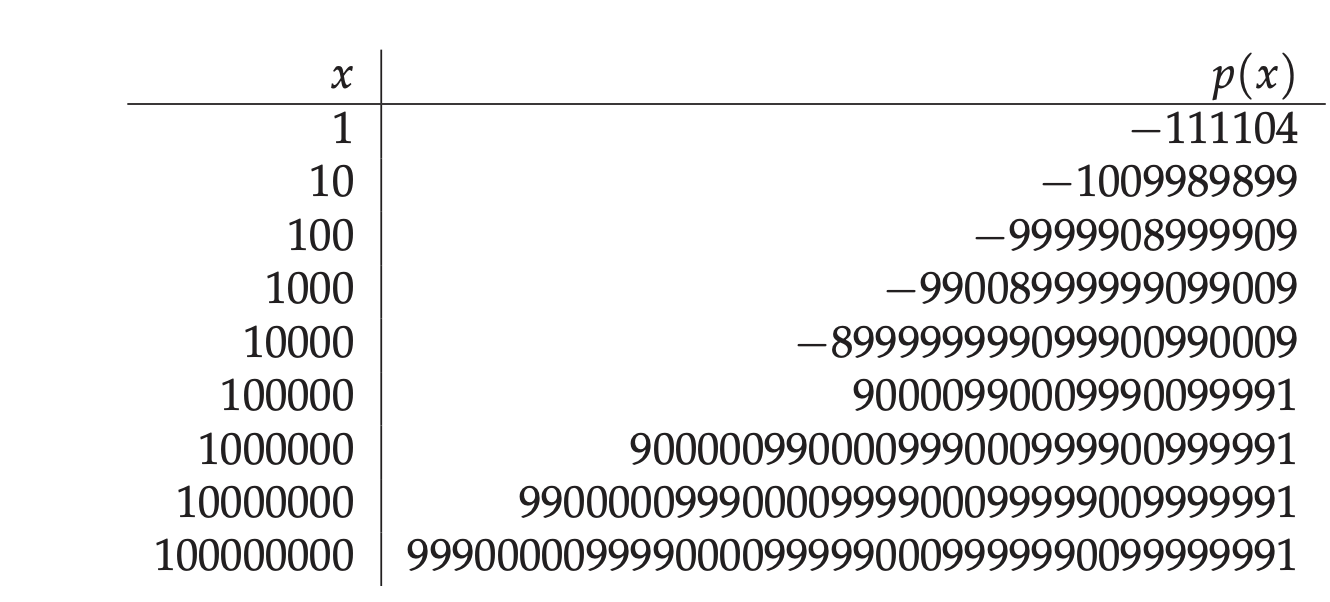
\includegraphics[scale=0.2]{at-infty.png}
\end{figure}
To analyze the behavior as \(x\to\pm\infty\), factor out the highest degree term.
If \(c\,x^n\) is the highest degree term in \(p(x)\), then for very large \(|x|\), \(p(x)\) behaves like \(c\,x^n\).

\subsection{Zero in an Interval}
\subsubsection{Intermediate Value Theorem}
Suppose \(p\) is a polynomial and \(a, b \in \mathbb{R}\) with \(a < b\). If \(p(a)\) and \(p(b)\) have opposite signs, then there exists a number \(c \in (a, b)\) such that \(p(c)=0\).

\subsection{Example 7: Zero in an Interval}
Let
\[ p(x) = x^5 + x^2 - 1. \
Explain why \(p\) has a zero in the interval \((0,1)\).
Solution:
Evaluate the polynomial at the endpoints:
\[ p(0) = 0^5 + 0^2 - 1 = -1 \quad \text{and} \quad p(1) = 1^5 + 1^2 - 1 = 1. \
Since \(p(0) < 0\) and \(p(1) > 0\), by the Intermediate Value Theorem, there exists a \(c \in (0,1)\) such that \(p(c)=0\).

\subsection{Zeros for Polynomials with Odd Degree}
Every polynomial with odd degree has at least one real zero.
For a polynomial \(p(x)\) of odd degree, as \(x \to -\infty\), \(p(x)\) tends to \(-\infty\) (or \(+\infty\)) and as \(x \to \infty\), \(p(x)\) tends to \(+\infty\) (or \(-\infty\)).
By the Intermediate Value Theorem, since \(p(x)\) changes sign, there exists at least one real number \(c\) such that \(p(c)=0\).

\section{Rational Function}
\subsection{Definition}
A \emph{rational function} is a function \(r\) defined by
\[ r(x) = \frac{p(x)}{q(x)}, \
where \(p(x)\) and \(q(x)\) are polynomials, with \(q(x) \neq 0\).

\subsection{Domain of a Rational Function & Example for \(r(x)\)}
The domain of a rational function
\[ \frac{p(x)}{q(x)} \
is the set of all real numbers where the expression makes sense. Since division by 0 is undefined, we exclude all zeros of \(q(x)\).

\subsubsection{Example}
\[r(x)=\frac{3x^5+x^4-6x^3-2}{x^2-9}\]
Factor the denominator:
\[ x^2-9=(x-3)(x+3). \
Thus, \(r(x)\) is undefined at \(x=3\) and \(x=-3\). Hence, its domain is
\[ \{x\in\mathbb{R}: x\neq 3 \text{ and } x\neq -3\}. \

\subsubsection{Example}
\[s(x)=\frac{x^3-6x+5}{x^4+9}\]
The denominator \(x^4+9\) is always positive (since \(x^4\ge 0\) and \(9>0\)). Therefore, \(s(x)\) is defined for every real number.
Domain of \(s(x)\) :
\( \mathbb{R} \

\subsection{Advantages of Mixed Representation}
Expressing a rational function as a polynomial plus a proper rational function (one where the numerator's degree is less than the denominator's) is analogous to writing an improper fraction as an integer plus a proper fraction.
\begin{itemize}
  \item \textbf{Simplification:} It makes further operations (such as integration, differentiation, and partial fraction decomposition) easier.
  \item \textbf{Asymptotic Insight:} The polynomial part reveals the behavior of the function as \(x\to\pm\infty\), while the proper fraction (the remainder) tends to zero for large \(|x|\).
  \item \textbf{Clarity:} It separates the "whole" part from the "fractional" part, making the function's structure more transparent.
\end{itemize}

\subsection{Mixed Rational Function Representation}
Express
\[ \frac{x^5 + 6x^3 + 11x + 7}{x^2+4} \
in the form
\[ G(x) + \frac{ax+b}{x^2+4}, \
where \(G(x)\) is a polynomial and \(a, b\) are constants.

\subsection{Procedure for Dividing Polynomials}
\begin{enumerate}
  \item \textbf{Rewrite:} Express the highest-degree term in the numerator as a single term times the denominator, plus the necessary adjustment.
  \item \textbf{Simplify:} Use the rewritten numerator to simplify the quotient.
  \item \textbf{Iterate:} Repeat steps (1) and (2) on the remaining rational function until the degree of the numerator is less than the degree of the denominator or the numerator becomes 0.
\end{enumerate}

\subsection{Mixed Representation Example}
Express
\[ \frac{x^5+6x^3+11x+7}{x^2+4} \
in the form
\[ G(x)+\frac{ax+b}{x^2+4}, \
where \(G(x)\) is a polynomial and \(a, b\) are constants.
\subsubsection{Step 1: Eliminate the \(x^5\) Term}
Notice that
\[ x^5=x^3(x^2+4)-4x^3. \
Therefore,
\[
\begin{aligned}
  x^5+6x^3 &= x^3(x^2+4)-4x^3+6x^3\\[1mm]
           &= x^3(x^2+4)+2x^3.
\end{aligned}
\]
So we can write:
\[ \frac{x^5+6x^3+11x+7}{x^2+4}=x^3+\frac{2x^3+11x+7}{x^2+4}. \

\subsubsection{Step 2: Eliminate the \(2x^3\) Term}
Write
\[ 2x^3=2x(x^2+4)-8x. \
Then,
\[
\begin{aligned}
  2x^3+11x+7 &= 2x(x^2+4)-8x+11x+7\\[1mm]
              &= 2x(x^2+4)+(3x+7).
\end{aligned}
\]
Thus,
\[ \frac{2x^3+11x+7}{x^2+4}=2x+\frac{3x+7}{x^2+4}. \

\subsubsection{Final Mixed Representation}
Combining the steps, we have:
\[ \frac{x^5+6x^3+11x+7}{x^2+4}=x^3+2x+\frac{3x+7}{x^2+4}. \

\subsection{Division Algorithm for Polynomials}
If \(p(x)\) and \(q(x)\) are polynomials with \(q(x) \neq 0\), then there exist unique polynomials \(G(x)\) and \(R(x)\) such that
\[ \frac{p(x)}{q(x)} = G(x) + \frac{R(x)}{q(x)}, \
where either \(R(x)=0\) or \(\deg R < \deg q\). Equivalently, we can write
\[ p(x)=q(x)G(x)+R(x). \

\subsection{Division by \(x-t\) and Zeros of a Polynomial}
Fix a real number \(t\) and let \(q(x)=x-t\). Since \(\deg q=1\), the remainder \(R(x)\) is a constant \(c\)(Because degree \(R < \)degree \(q\)). Thus, there exist a polynomial \(G(x)\) and a constant \(c\) such that
\[ p(x) = (x-t)G(x) + c. \
Evaluating at \(x=t\) yields \(p(t)=c\), so we can rewrite this as
\[ p(x) = (x-t)G(x) + p(t). \
\(t\) is a zero of \(p\) if and only if \(p(t)=0\), which happens precisely when
\[ p(x)=(x-t)G(x). \

\subsection{Behavior of a Rational Function Near \(\pm\infty\)}
To determine the behavior of a rational function as \(x\to\pm\infty\), factor out the highest power of \(x\) in the numerator and the denominator.
Consider
\[ r(x)=\frac{9x^5-2x^3+1}{x^8+x+1}. \
The highest degree in the numerator is \(x^5\) and in the denominator is \(x^8\). Factoring these out yields:
\[ r(x) \sim \frac{9x^5}{x^8}=\frac{9}{x^3}. \
As \(|x|\) becomes very large:
\begin{itemize}
  \item \(r(x)\to 0\) as \(x\to\infty\) (approaching \(0^+\)).
  \item \(r(x)\to 0\) as \(x\to-\infty\) (approaching \(0^-\)).
\end{itemize}

\subsection{Asymptote of a Rational Function}
A line is an asymptote of a graph if the graph becomes and stays arbitrarily close to the line as \(x\) tends to \(\pm\infty\).
Consider
\[ r(x)=\frac{3x^6-9x^4+6}{2x^6+4x+3}. \
Both the numerator and the denominator are degree 6. Therefore, the horizontal asymptote is the ratio of the leading coefficients:
\[ y=\frac{3}{2}. \
\begin{figure}
\centering
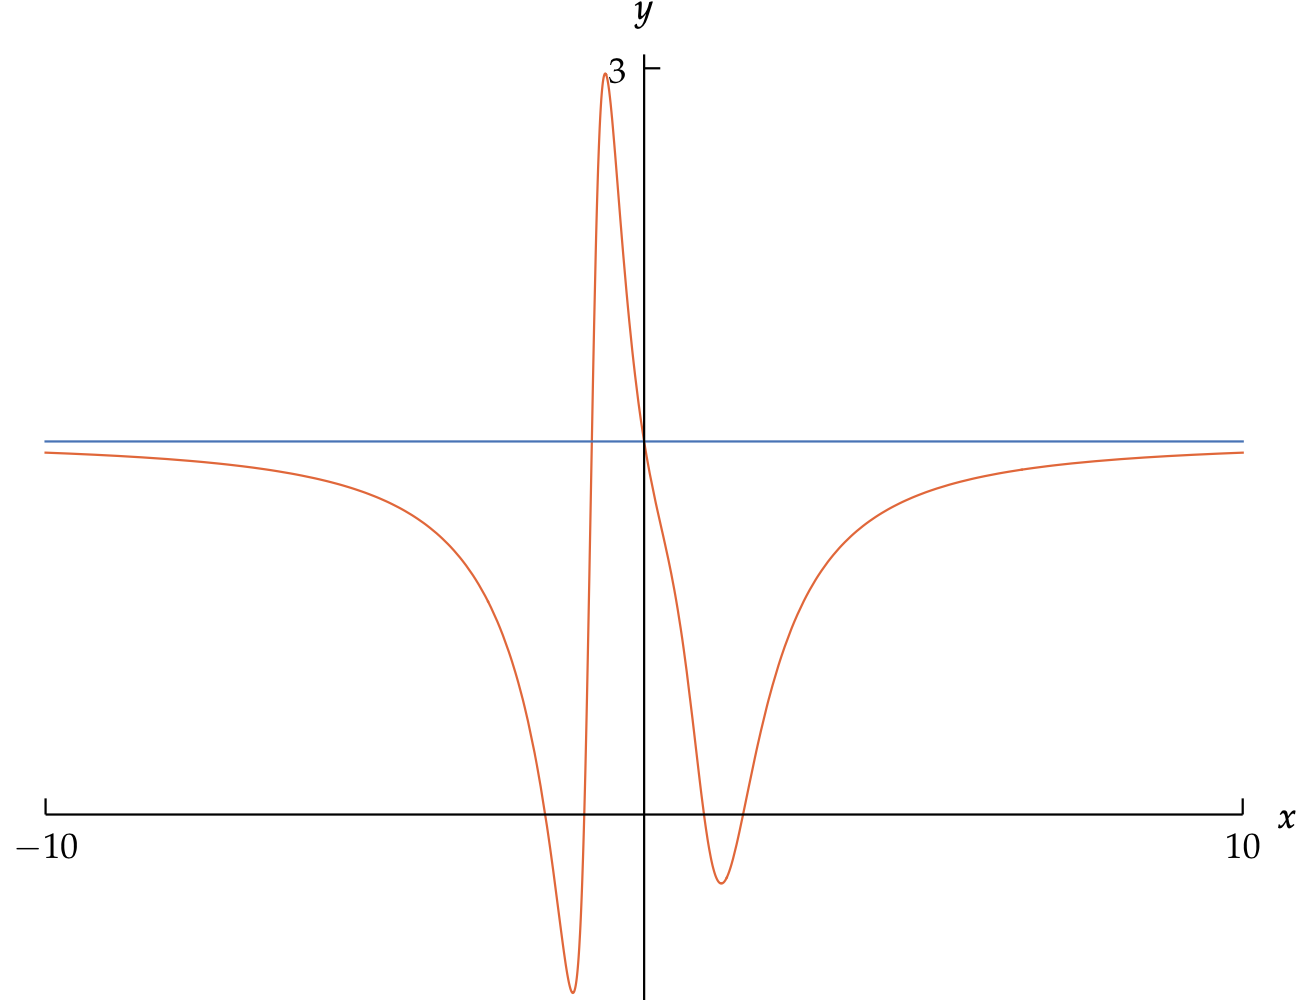
\includegraphics[scale=0.2]{asymptote1.png}
\end{figure}

\subsubsection{Example}
\[ r(x) = \frac{4x^{10}-2x^3+3x+15}{2x^6+x^5+1} \
Solution:
\[ \frac{4x^{10}}{2x^6} = 2x^4. \
Thus, as \(|x|\to\infty\), \(r(x)\) behaves like \(x^{4}\). That is, \(r(x)\) is very large and positive when \( x \to \infty\) and \( x \to -\infty\).
